% --------------------------------------------------------------------------
% Report template for BIR projects
% Report template with support for Portuguese and English languages
% Change language {brazil or english} in \documentclass as per the examples
% This template has support for the ABNT citing format
% 
% Original version: jan/2019
% https://github.com/
% 
% Based on ABNTEX2 and the thesis template
% --------------------------------------------------------------------------
\documentclass[
%\DeclareUnicodeCharacter{200B}{}
% --------------------------------------------------------------------------
% classe memoir . options                                                   
12pt,					% tamanho da fonte
openright,				% cap. começam em pág ímpar (ins pág vazia caso preciso)
twoside,				% para impressão em verso e anverso. Oposto a oneside
a4paper,				% tamanho do papel
% --------------------------------------------------------------------------
% classe abntex2 . options                                                  
%chapter=TITLE,			% títulos de capítulos convertidos em letras maiúsc.
%section=TITLE,			% títulos de seções convertidos em letras maiúsc.
%subsection=TITLE,		% títulos de subseções convertidos em letras maiúsc.
%subsubsection=TITLE,	% títulos de subsubseções convertidos em letras maiúsc.
% --------------------------------------------------------------------------
% Opções de IDIOMA do pacote babel                                          
english,
brazil
]{ABNT/abntex2_report}
% --------------------------------------------------------------------------
% Pacotes básicos    
\usepackage{lmodern}			% Usa a fonte Latin Modern			
\usepackage[T1]{fontenc}		% Selecao de codigos de fonte.
\usepackage[utf8]{inputenc}		% Codificacao do documento (conversão automática dos acentos)
\usepackage{indentfirst}		% Indenta o primeiro parágrafo de cada seção.
\usepackage{color}				% Controle das cores
\usepackage{graphicx}			% Inclusão de gráficos
\usepackage{microtype} 			% para melhorias de justificação
\usepackage{lipsum}	
\usepackage[brazilian,hyperpageref]{backref} % páginas com citações na bibliog.
%\usepackage[alf,abnt-etal-list=0,abnt-etal-cite=3,abnt-emphasize=bf]{abntex2cite}
\usepackage[alf]{abntex2cite}
%	
\usepackage{lastpage}			% Usado pela Ficha catalográfica
%\usepackage{subfig}
\usepackage{supertabular}       % tabela na capa do documento
\usepackage{booktabs}
\usepackage[table,xcdraw]{xcolor}
\usepackage{adjustbox}
\usepackage{amssymb,amsmath,mathrsfs}
\usepackage{algorithm,algpseudocode}
\usepackage{pgfplots}
\usepackage{tikz}
\usepackage{titlesec}
\usepackage{ragged2e}
\usepackage{tocloft}
\usepackage{threeparttable}
\usepackage{etoolbox}
\usepackage[normalem]{ulem}
\usepackage{yaacro}
\usepackage[none]{verlab}
%\usepackage{fontspec}
%\setmainfont{Helvetica Light}
\usepackage{lscape}
%\usepackage[graphicx]{realboxes}
\usepackage{rotating}
\usepackage{wrapfig}
\usepackage{caption}
\usepackage{subcaption}
\usepackage{dirtytalk}
\usepackage{pdfpages}
\usepackage{threeparttable}
\usepackage{hyperref}
%\hypersetup{draft}
\usepackage{float}
\DeclareUnicodeCharacter{200B}{}
% --------------------------------------------------------------------------%
% Configurações do PDF final                                                
\definecolor{blue}{RGB}{41,5,195}
\makeatletter
\hypersetup{
	%pagebackref=true,
	pdftitle={\@title}, 
	pdfauthor={\@author},
	pdfsubject={\@title},
	%pdfsubject={\imprimirpreambulo},
	pdfcreator={LaTeX with abnTeX2},
	pdfkeywords={abnt}{latex}{abntex}{abntex2}{\imprimirpalavraschave}, 
	colorlinks=true,       		% false: boxed links; true: colored links
	linkcolor=blue,          	% color of internal links
	citecolor=blue,        		% color of links to bibliography
	filecolor=magenta,      	% color of file links
	urlcolor=blue,
	bookmarksdepth=4
}
%\makeatother
% --------------------------------------------------------------------------
% Posiciona figuras e tabelas no topo da página quando adicionadas sozinhas
% em um página em branco. Ver https://github.com/abntex/abntex2/issues/170
%\makeatletter
\setlength{\@fptop}{5pt} % Set distance from top of page to first float
\makeatother
% --------------------------------------------------------------------------
% Formatação                                                                
\newcommand\tab[1][1cm]{\hspace*{#1}}
\apptocmd{\thebibliography}{\justifying}{}{} 
\renewcommand{\ABNTEXsectionfont}{\bfseries}
\titlespacing*{\chapter}{0pt}{0pt}{12pt}
\titlespacing*{\section}{0pt}{6pt}{6pt}
\titlespacing*{\subsection}{0pt}{6pt}{6pt}
\titlespacing*{\subsubsection}{0pt}{6pt}{6pt}
% --------------------------------------------------------------------------
% Rearranja os finais de cada estrutura                                     
\algrenewtext{EndWhile}{\algorithmicend\ \algorithmicwhile}
\algrenewtext{EndFor}{\algorithmicend\ \algorithmicfor}
\algrenewtext{EndIf}{\algorithmicend\ \algorithmicif}
\algrenewtext{EndFunction}{\algorithmicend\ \algorithmicfunction}
% --------------------------------------------------------------------------
% Espaçamentos entre linhas e parágrafos                                    
\setlength{\parindent}{1.3cm} % linha
\setlength{\parskip}{0.2cm} % parágrafo, tente também \onelineskip
% --------------------------------------------------------------------------
% Informações de dados para CAPA e FOLHA DE ROSTO                           
\prodtecnica{001 / 2020}
\titulo{Superapresentações- COMO VENDER IDEIAS E CONQUISTAR AUDIÊNCIAS}
% \tiporelatorio{Parcial} 
% \nomeprojeto{Resumo}
\outrossubtitulos{~} % opcional
\autores{
	Eduardo Adas \\
	Joni Galvao\
}
\newcommand{\autoresexternos}{
	Jéssica Motta
}
\local{Salvador\\Bahia, Brasil}
\data{Junho de 2020}
% \classificacao{( ) Confidencial  (X) Restrito  ( )  Uso Interno  ( ) Público}
% \revisao{01}
% \tabelacutter{000} 
% \palavraschave{1. Manipulator. 2. Simulation. 3. Computer vision.}
% \classificacaoassunto{000} % Número de Classificação do assunto 
%\parceirologo{logos/x.png}
%------------------------------------------------------------------
% Finalização das configurações da capa
%
%
%------------------------------------------------------------------              
% Acrônimos :: Chamar no texto como \ac{DoF}                                
\begin{acgroupdef}[list=acronyms]
	\acdef{DoF}{Degrees of Freedom}
	\acdef{PoC}{Proof of Concept, em português Prova de Conceito}
	\acdef{UUV}{Unmanned Underwater Vehicle, em português Veículo Subaquático Não-tripulado}
	\acdef{AUV}{Autonomous Underwater Vehicle, em português Veículo Subaquático Autônomo}
	\acdef{UVM}{Unmanned Vehicle Morphing}
	\acdef{SLAM}{Simultaneous Localization and Mapping}
	\acdef{ROV}{Remotely Operated Vehicle}
	\acdef{SOTA}{Study Of The Art}
	%
	%
	%
\end{acgroupdef}
% --------------------------------------------------------------------------
% Criação do sumário
\makeindex
%
\begin{document}
	\frenchspacing
	\imprimircapa
	% \imprimircatalografica
% --------------------------------------------------------------------------
% % Sumário executivo                                                         
% 	\ABNTEXchapterfont\large\textbf{\execsummarytitlename}
% 	\begin{flushleft}
% 		\normalsize
% 		\justify
% 		\normalfont
% 		O projeto de Manipuladores - Desafio.2, também conhecido como \textbf{xxxxx} se configura sob o Programa de Formação de Novos Talentos do Serviço Nacional de Aprendizagem Industrial, Departamento Regional da Bahia - Senai/DR/BA, sendo este o principal fomentador do programa.

% 		O projeto foi considerado como início técnico do projeto o dia 00 de bolsoneiro de 2020. 

% 		O prazo de execução planejado é de xx meses.
% 	\end{flushleft}
% 	\clearpage
%------------------------------------------------------------------
% Resumo e abstract                                                         
	\ABNTEXchapterfont\large\textbf{\resumoatitlename}
	\begin{flushleft}
		\normalsize
		\justify
		\normalfont
		Este resumo tem por finalidade trazer os pontos chaves do livro Superapresentações- COMO VENDER IDEIAS E CONQUISTAR AUDIÊNCIAS, para ajudar estagiários, bolsistas e profissionais do laboratório RoSA (Robótica e Sistemas Autônomos) a construirem apresentações incríveis e venderem suas ideias.
	\end{flushleft}
	\vspace*{1cm}
	\newpage
	% %
	% \ABNTEXchapterfont\large\textbf{\resumobtitlename}
	% \begin{flushleft}
	% 	\normalsize
	% 	\justify
	% 	\normalfont
	% 	%abstract aqui
	% 	%
	% 	%
	% 	%
	% \end{flushleft}
	\clearpage
% --------------------------------------------------------------------------
% Lista de figuras                                                          
	% \begin{flushleft}
	% 	\ABNTEXchapterfont\Large\textbf{\MakeUppercase\listadefigurasname}
	% \end{flushleft}
	% \vspace*{-36pt}
	% \pdfbookmark[0]{\listfigurename}{lof}
	% \normalsize
	% \listoffigures*
	% \cleardoublepage
% --------------------------------------------------------------------------
% % Lista de tabelas                                                          
% 	\begin{flushleft}
% 		\ABNTEXchapterfont\Large\textbf{\MakeUppercase\listadetabelasname}
% 	\end{flushleft}
% 	\vspace*{-36pt}
% 	\pdfbookmark[0]{\listtablename}{lot}
% 	\normalsize
% 	\listoftables*
% 	\cleardoublepage
% --------------------------------------------------------------------------
% % Lista de símbolos e abreviaturas                                          
% 	\begin{flushleft}
% 	\ABNTEXchapterfont\Large\textbf{\MakeUppercase\listadesimbolsabrevtitlename}
% 		\noindent
% 		\vspace*{-06pt}
% 		\pdfbookmark[0]{\listadesiglasname}{lot}
% 		\normalsize
% 		\normalfont
% 		\aclist[list=acronyms]
% 	\end{flushleft}
% 	\newpage
% --------------------------------------------------------------------------
% Tabela de conteúdo                                                        	
	\begin{flushleft}
		\ABNTEXchapterfont\Large\textbf{\MakeUppercase\glosariotitlename}
	\end{flushleft}
	%\pagebreak
	\vspace*{-36pt}
	\pdfbookmark[0]{\contentsname}{toc}
	\normalsize
	\normalfont
	\tableofcontents*
	\justify
% --------------------------------------------------------------------------
% Formatação, remover espaço depois dos títulos
	\setlength\beforechapskip{-24pt}
	\setlength\afterchapskip{12pt}
	\textual
	\pagestyle{plain}
	\normalsize
	\justify
	\normalfont
% --------------------------------------------------------------------------
% Conteúdo do relatório  
	\chapter{PONTOS CHAVES}
\label{chap:keypoints}
\begin{itemize}
    \item É preciso que o cliente visualize o valor do negócio que você está vendendo
    \item Sempre se reinventar 
    \item Avaliações internas, pesquisa de satisfação dos clientes etc.
    \item Fazer as seguintes perguntas: "usaremos metáforas ou analogias? O ouro será entregue no início ou no final? Quais serão as principais emoções incorporadas a essa história? Que recursos visuais e de linguagem usaremos para impactar a audiência?"
    \item Equilibrio entre razão e emoção acompanhada de uma linguagem visual sofisticada a partir de uma visão estratégica da comunicação em apresentações e coerente com o estilo do cliente
    \item Conhecer a audiência para preparar uma apresentação para esta, pesquisar no site da empresa, chegar antes do horário para conversar com pessoas e identificar a dinâmica local, fazer perguntas no início da apresentação para identificar se precisa aprofundar em alguns conceitos ou passar rápido por outros ou até mesmo improvisar
    \item Necessário criar um vínculo emocial com a audiência
    \item A apresentção precisa impactar, encantar e imprimir uma mensagem na audiência até levá-la à ação
    \item É a mídia dos 30 segundos
    \item A principal maneira de comunicar ideias é através de apresentações
    \item Objetivo da apresentação é levar a audiência a aderir algo seja: um produto, um conceito ou mesmo uma mudança de comportamento
    \item Uma apresentação SOAP é conduzida por uma história coerente, bem estruturada e atraente
    \item A história deve revelar uma mensagem principal, valorizá-la e sustentá-la com bons argumentos
    \item A mensagem principal deve representar um benefício para a audiência
    \item O apoio visual deve reforçar as mensagens presentes no discurso do apresentador
    \item SOAP alinha todos os aspectos citados por meio de soluções de comunicação criativas e impactantes
    \item 1- Diagnóstico em torno da apresentação; 2- confecção de um roteiro;  3- desenvolvimento de apoio visual e 4- treinamento do apresentador
    \item Em apresentações corporativas as histórias não devem roubar o espaço de dados importantes
    \item Apresentações para públicos menores custam ser intimistas, com uma abordagem mais pessoal
    \item Para públicos maiores é necessário ter cuidado com dimensões das fontes e das imagens que ilustram os slides.
    \item Tempo: palestras e eventos possuem tempo predeterminado, no caso de reuniões perguntar quanto tempo disponível as pessoas têm e verificar se a pessoa essencial para a aprovação do projeto quer detalhamento do projeto ou se será necessário omitir algumas coisas
    \item Apresentador: o tom da apresentação deverá ser de acordo com o perfil do apresentador: mais sério ou mais desinibido
    \item A ousadia na apresentação é bem vinda desde que compatível com o perfil do apresentador, se a apresentação ousada não é compatível com este é necessário que treine até que tenha incorporado o roteiro.
    \item A partir do objetivo identificado que irá brotar o tema da apresentação, aquele que servirá de base para o desenvolvimento de todo o roteiro.
    \item A apresentação deve mesclar razão, emoção, conteúdo e entretenimento
    \item deve garantir: interesse imediato da audiência, a manutenção da atenção e o entendimento das mensagens
    \item  O discurso deve ser centrado na audiência
    \item A mensagem principal: deve trazer benefício para sua audiência (foque nisso)
    \item Mensagens de suporte: sustentam a mensagem principal, dependendo do contexto podem ser positivas ou negativas. Caso estas não estejam a serviço da principal avalie se são mesmo relevantes
    \item Slogan: título ou chamada da matéria, devido ao destaque este fica na mente da audiência,
    \item Estruturação de raciocínio: a sequência dos slides culminam em determinada conclusão
    \item Inserção do conteúdo: depois de criar a história é inserido o conteúdo de forma a sustentá-lo (números, dados, casos de sucesso e outras informações relevantes), um conteúdo impactante precisa ser consistente, objetivo e conciso
    \item Caso tenha muitos dados para mostrar a audiência e nenhuma história para contar, mande tudo por e-mail
    \item No contexto da história dê foco apenas aos números mais importantes, se os números forem vários entregar para a audiência um documento a parte
    \item Adequação da linguagem: ser conciso e facilitar a compreensão da audiência sem distorções
    \item Direto ao ponto: revela a mensagem principal nos primeiros minutos- usado para pessoas que tem agenda atribulada e pouco tempo. Quando a pessoa já conhece o tema a ser tratado e deseja se aprofundar mais no assunto, também quando os ouvintes são sabidamente ansiosos e inquietos, ou quando uma notícia ruim precisa ser revelada (dedicar o tempo a breves justificativas e propostas de reverter o cenário).
    \item Metáfora: usada para audiência leiga e quando há a necessidade de transmitir conceitos técnicos, quando bem empregadas geram identificação entre uma audiência e um tema
    \item Suspense: usada apenas quando se tem uma boa notícia para dar, uma bonificação, uma vitória diante de uma concorrência
    \item Surpresa: uma imagem divertida ou passagens atraentes no geral cria a expectativa na audiência que o apresentador pode surpreendê-la
    \item Conflito x solução: chamar a atenção da audiência para determinado problema, envolvê-la nos pormenores e mostrar-lhe uma solução
    \item Humor: não é contar piadas e sim inserir passagens divertidas, o humor funciona bem com pessoas naturalmente engraçadas,boa alternativa é usar a autoironia, se expor e criar empatia e estreitar a comunicação, se o apresentador não for naturalmente engraçado- usar vídeos ou imagens engraçadas coerentes com o roteiro
    \item Questionamento: levantar questionamento durante a apresentação gera inquietação mental e corporal
    \item Drama: depois de revelado o drama o apresentador mostra uma proposta de mudança de abordagem
    \item Tom provocativo: baseia-se em comentários e questionamentos sobre os pontos fracos da audiência e logo após oferece-se soluções de melhorias
    \item A primeira impressão é o gatilho para empatia ou desinteresse
    \item A primeira tela deve ter uma imagem, slogan ou até um questionamento que gere expectativa à audiência
    \item 3 atos da apresentação: ato 1: revelar logo ou deixar um ar de suspense sobre o que será tratado; ato 2- é 90\% do tempo da apresentação deve responder: quem?(ou o quê?), quando? onde? quanto? como? por quê? para quê? ato 3: consolida a mensagem principal
    \item Foco no que é relevante 
    \item Nível de detalhamento- evitar atirar para todos os lados, ter claro os objetivos em cada transação, para maiores detalhamentos marque outra reunião ou mande-os por email
    \item Informações precisam impactam a audiênciaa
    \item Tornando um fato palpável ajuda a audiência a reter a informação
    \item Evite se elogiar, dê foco ao produto ou ao projeto, os elogios formulados pela audiência têm muito mais impacto
    \item As mensagens visuais e verbais devem ser assertivas não dando margem para outras interpretações
    \item Estruture uma agenda da apresentação a partir da identificação dos temas para fragmentar o roteiro. Uso de tela de transição para situar a audiência
    \item Decidir o que vai para o slide e o que vai para o discurso, para o slide (imagens, palavras-chaves, ou sentenças breves)
    \item A fala do apresentador em uma apresentação composta de imagens e palavras-chaves passa confiança e credibilidade ao público
    \item Eleja a mensagem que quer passar naquele slide e ilustre-a da melhor maneira
    \item a quantidade de slides vai depender de cada apresentador e ele que dita o ritmo de apresentação não a quantidade de slides
    \item Fugir de textos grandes independente do contexto ou abordagem
    \item Pensar em como quer que a mensagem chegue a audiência e a sequência entre discurso e imagem
    \item cada slide deve ser pensado individualmente
    \item O ideal é que os slides possam ser decifrados em no max 5 segundos para que o público capte a mensagem principal sem se desconectar do seu discurso
    \item Não usar efeitos nos textos, irrita o público
    \item Escolher as imagens conforme as emoções que se deseja provocar no público. válido o uso de imagens, ícones, grafismos, montagens
    \item Atenção a estética na construção dos slides, ser humano procura padrões e alinhamentos, as imagens devem estar alinhadas no slide
    \item usar as linhas de orientação visual para colocar as imagens no slide
    \item Importante confeccionar um slide de apresentação e uma tela de espera
    \item Se achar adequado o apresentador pode mostrar alguns conceitos na introdução e só em seguida revelar o tema e a capa, esta será o desfecho da introdução
    \item A tela de descanso é usada antes da apresentação começar e já antecipa a mensagem principal que será passada
    \item Usar os bullets points com parcimônia (na exposição da agenda da apresentação, na sintese de pontos que foram abordados anteriormente, para relacionar funções ou características de um produto ou serviço, para rever passos de um projeto)
    \item Se for necessário ter muitas informações no slide, chame atenção para as informações mais relevantes
    \item Deixar os dados extras em documento a parte para ficar em mãos e consultar caso necessário
    \item Criar uma identidade visual é importante para associar a marca ou tema, manter uma homogeneidade nos slides
    \item Uso de tons que tenham distinção sutis ou cores complementares que causam maior impacto, rosa com verde, laranja com azul
    \item Verificar as cores que estão relacionados com o tema ou marca. Ex.: Petrobras apresentações nacionais usa verde e amarelo e nas internacionais azul 
    \item Fontes: Arial ou Helvetica, Trebuchet ou Century Gothic. Títulos: 20 a 25 e textos corridos 16 a 18, se for uma plateia de mais de 200 pessoas usar 18 como mínimo. Cuidado ao usar letras em maiusculo para não atrabalhar a leitura de textos
    \item Linhas: ângulos agudos e pontas denotam tensão, tecnologia, formalidade; linhas curvas e suaves: expressam mais leveza e criatividade; linhas verticais sequenciais: revelam organização e certa rigidez. Servem para dar ênfase, emoldurar imagens e até delimitar margens. Presenter Pro 
    \item o uso de formas fazer o mesmo trabalho das linhas
    \item Fundo de página branco ou preto
    \item Fuja dos templates e da inserção da logo em todos os slides, acabam por poluir a apresentação
    \item Elementos gráficos ajudam a compor a identidade visual dos slides
    \item As fotos são âncoras, estímulos externos provocam sensações e emoções ao público, saiba o que quer passar à eles. Conexões positivas são melhores.
    \item Foto- objeto: são fotos recortadas, sem fundo, usada para quem faz apresentação com poucos recursos
    \item Clip-art: em apresentações corporativas fuja delas, acabam por banalizar a apresentação, e fica difícil surpreender a audiência
    \item ícones customizados: não quer grandes habilidades artísicas 
    \item Fonte como imagem; transfere uma mensagem além da verbal, exemplo "reservatórios de água" com letras vazadas qiue mostrem por trás um volume de água reduzindo gradativamente da primeira á última letra
    \item Desenhos e ilustrações: quanto mais humanos os desenhos, mais humana a resposta à eles. A combinação dos desenhos feito à mão e no computador ajudam a estruturar uma boa apresentação
    \item Depois de estar com o roteiro, slide e mensagem principal prontos é hora de treinar o texto até que tenha se tornado um contador de histórias, é importante atentar para o tom de voz e as expressões se quer fazer o público focar em você
    \item O apresentador pode começar a introduzir um conceito e daí passar para o slide com essa informação, isso gera suspense, mas para esse timing funcionar é preciso que o apresentador esteja afinado com a apresentação e saiba a sequência de slides
    \item Estar atento ao tempo de apresentação, lembrando de deixar tempo reservado a perguntas, atividades e intervalos. Se necessário até levar um alarme no bolso nos 10 a 15 min finais
    \item Conheça sua platéia 
    \item Usar linguagem de bate-papo com os amigos, evitando jargões, clichês e abordagens negativas
    \item Dê uma margem para improviso, tenha um pequeno repertório e use conforme feeling em relação a audiência e tempo, contando uma experiência pessoal ou de terceiros
    \item fala: entonação e melodia- sem variações de entonação fica entendiante, mas cuidado para não soar forçado, isso depõe contra você; volume- fale de forma a ser ouvido, e varie o volume afim de chamar atenção para alguns trechos, mesmo que esteja usando o microfone; clareza- articule bem as palavras; ênfase- a ênfase em uma ou outra palavra pode mudar o foco da mensagem; pausas- são bem-vindas, usada para respirar, pensar no que vai falar, tempo para o público absorver o que acabou de ser dito e até criar expectativa ao que será dito; velocidade do discurso- falas apressadas criam ansiedade e lentas de mais cansaço na audiência; o tom do discurso- deve estar condizente ao que será dito, indignação não pode ser dita de forma suave, nem demonstrar controle de uma situação em tom desesperador; cuide da sua voz- beba bastante água  
    \item Não force entusiasmo, seja autêntico, conte vivências pessoais relacionadas ao que está sem apresentado isso estreitará o elo com a audiência
    \item Foque o olhar na audiência, dê menos atenção aos slides e ao roteiro, estabeleça conexão com esta
    \item Uso de apresentador de slide e laser point ajuda na apresentação
    \item Ter uma versão elevador da apresentação é bem-vinda caso surja oportunidade em um voo ou algo similar, ter a versão resumida dos slides no celular
    \item Uso de apresentações autoexplicativas são bem-vindas quando se tem repetidos pedidos de demonstração e não têm pessoal suficiente disponível

\end{itemize}
%------------------------------------------------------------------




	% \chapter{CONCEITO DO SISTEMA}
\label{chap:conce}

	% \include{sections/03desenvolvimento}
	% \include{sections/04resultados}
	% \include{sections/05confiabilidade}
	% \include{sections/06conhecimento}
	% \include{sections/07conclusao}
	%\include{sections/02referencial}
	%\include{sections/03metodo}
% --------------------------------------------------------------------------
% Referências
	% \cleardoublepage
	% \titleformat{\chapter}[display]{\vspace*{-24pt}\ABNTEXchapterfont\large\bfseries}{\chaptertitlename\ \thechapter}{12pt}{\Large}
	% \bibliography{bibliography}
% --------------------------------------------------------------------------
% % Apêndices
% 	\apendices
% 	\justify
% 	%
% 	\chapter{Questões de abordagem à pesquisa}
% 	\label{apend:quest}
% 	%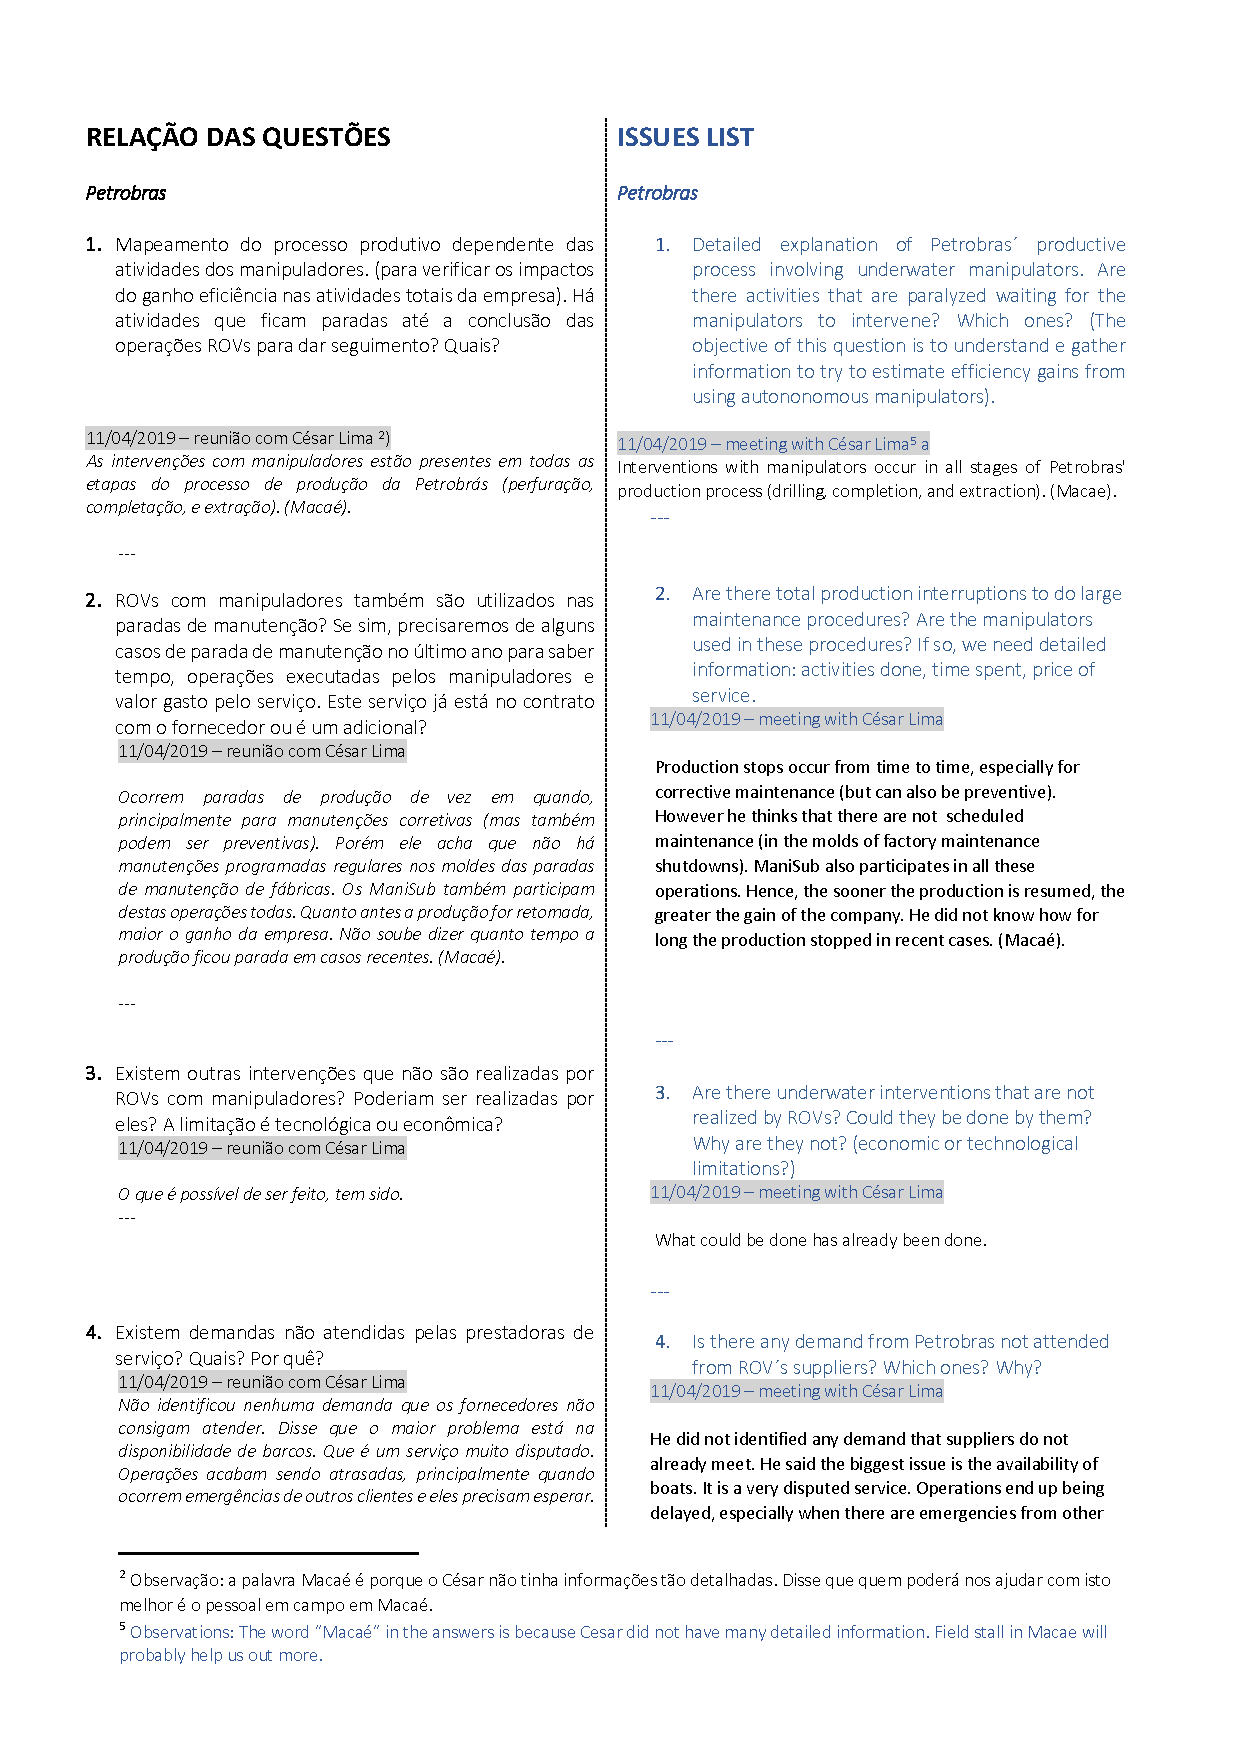
\includepdf[pages={{},-}]{appendix/listquest.pdf}
% 	\lipsum[1] % Comentar e adicionar apêndice aqui
% 	%
% 	\chapter{Um assunto importante}
% 	\label{apend:assunto}
% 	\lipsum[1] % Comentar e adicionar apêndice aqui
	

% --------------------------------------------------------------------------
% % Anexos                                                                     
% 	\anexos
% 	\justify
% 	%
% 	\chapter{Outro assunto importante}
% 	\label{ann:relant}
% 	%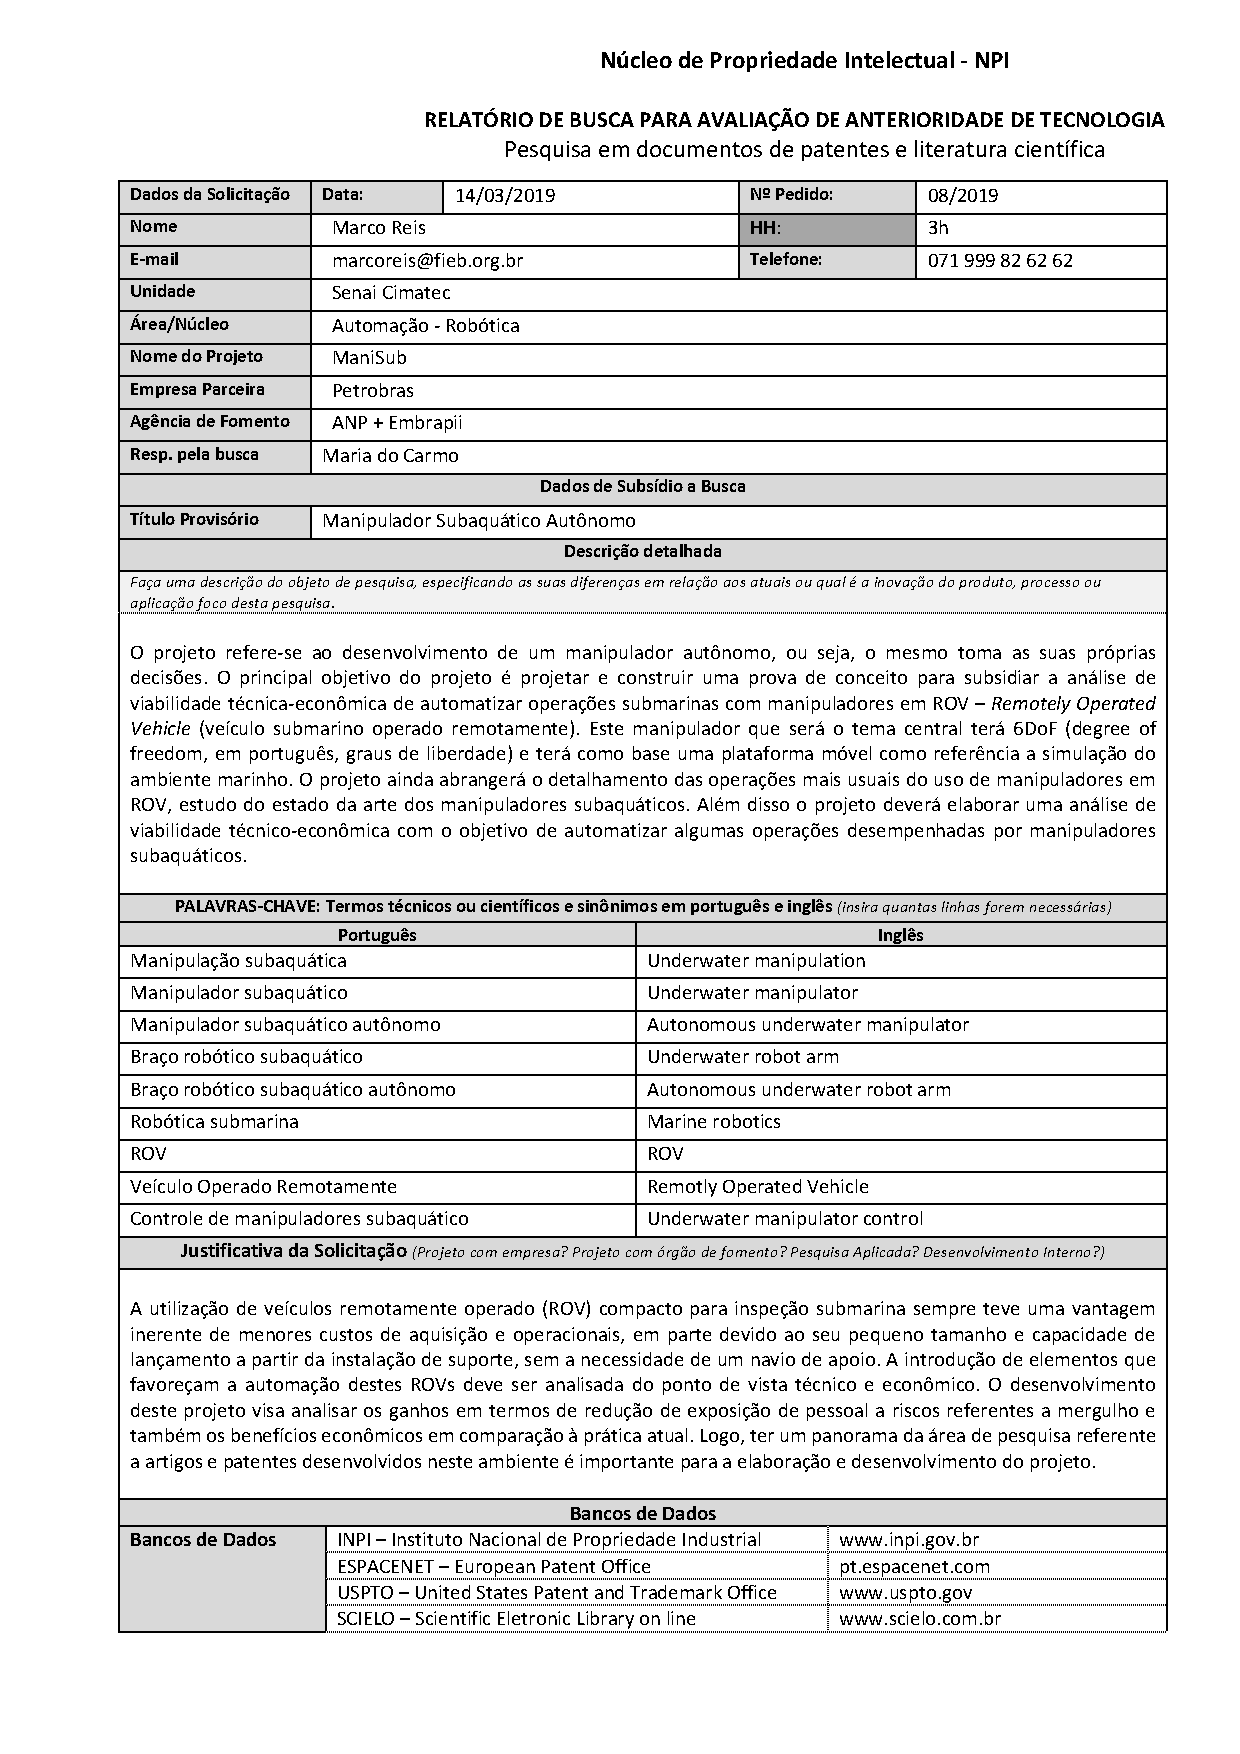
\includepdf[pages={{},-}]{annex/manisubanterioridade.pdf}
% 	\lipsum[1] % Comentar e adicionar apêndice aqui
% 	%
\end{document} 